\section{Inspektion}
Die \textbf{Inspektion} ist das komplizierteste, aufwändigste, fromalisierteste und \textit{effektivste Verfahren}, um Defekte manuell aufzuspüren (vgl~\cite[18]{Wed09c}).\\
Alle anderen Verfahren basieren auf dem Verfahren der Inspektion.\\

\noindent
Aufgrund ihres Aufwandes kommen Inspektionen in der Praxis i.d.R. nur bei \textit{sehr wichtigen} Prüfgegenständen zum Einsatz.\\

\noindent
Bei der Inspektion wird von \textbf{Gutachtern} die \textbf{Erfüllung der Spezifikation} und die \textbf{Einhaltung von Standards} geprüft.\\
Damit nichts Wichtiges übersehen wird, werden Checklisten verwendet, die nicht unbedingt umfangreich sein müssen.\\
Die Inspektion findet zunächst alleine durch die jeweiligen Gutachter statt.
Die Ergebnisse werden in einer anschließenden \textbf{Inspektionssitzung} besprochen.

\begin{tcolorbox}[colback=white]
    Die Erarbeitung von Möglichkeiten zur Behebung von Defekten ist kein Teil der Inspektion.
\end{tcolorbox}

\subsection{Inspektionsteam}

\begin{itemize}
    \item \textbf{Moderator}: organisiert die Vorgänge der Inspektion, moderiert die Inspektionssitzung.
    Hat im besten Fall bereits Erfahrungen mit Inspektionen gemacht und hat Kenntnisse in Gesprächsmoderation und strukturierter Arbeit mit Gruppen.
    \item \textbf{Autor(en)}: stehen während der Inspektion zur Beantwortung von Fragen zur Verfügung.
    \item \textbf{Inspektoren}: untersuchen den Prüfgegenstand, müssen also zu einer fachlichen Beurteilung in der Lage sein. Sind keine Vorgesetzten der Autoren.
    \item \textbf{Leser}: Einer der Inspektoren nimmt \textbf{während der Inspektionssitzung} die Rolle des \textbf{Lesers} ein, der durch den Prüfgegenstand führt.
\end{itemize}

\noindent
Wegen der Rollenverteilung \textbf{Leser}/\textbf{Inspektor} sollten mindestens zwei Inspektoren beteiligt sein.\\

\noindent
Das \textbf{Protokoll} führt der Moderator bei kleineren Inspektionsgruppen.\\
Bei größeren Gruppen (mehrere Inspektoren bzw. mehrere Autoren) übernimmt ein \textbf{dedizierter Protokollführer} diese Aufgabe.

\subsection{Ablauf}

\begin{enumerate}
    \item die Inspektion wird durch den \textbf{Autor} ausgelöst, indem er die Fertigstellung an den \textbf{Moderator} meldet
    \item die Eingangsmeldung wird vom \textbf{Moderator} überprüft (Vollständigkeit, formale Richtigkeit); daraufhin verteilt er den \textbf{Prüfgegenstand} and die \textbf{Inspektoren}; Termine für Einführungs- und Inspektionssitzung werden geplant
    \item der \textbf{Moderator} hält Rücksprache mit den \textbf{Inspektoren}, ob sie mit den Inhalten des Prüfgegenstandes genug vertraut sind; in dem Fall muss eine Einführungssitzung, in der der \textbf{Autor} in den Prüfgegenstand einführt, nicht zwingend stattfinden
    \item die \textbf{Inspektoren}, die keine Vorgesetzten der Autoren sein dürfen, untersuchen einzeln den Prüfgegenstand, ggfl. mit \textbf{Checklisten}
    \item einer der Inspektoren, der \textbf{Leser},  führt in der \textbf{Inspektionssitzung} systematisch durch den Prüfgegenstand; die Inspektoren tragen gefundene Defekte zusammen; der \textbf{Moderator} stellt sicher, dass keine Diskussionen über Behebungsmöglichkeiten entstehen, es finden nur Diskussionen statt, ob  es sich tatsächlich um Defekte handelt; die Dauer einer Inspektionssitzung ist auf max. $1.5$ - $3$h begrenzt
    \item eine \textbf{Freigabe} des Prüfgegenstandes erfolgt, falls nur wenige Defekte gefunden worden, und der \textbf{Moderator} die Behebung überprüft hat; gravierende Defekte bedingen eine erneute Inspektionssitzung
    \item die \textbf{Protokollierung} der Sitzungen übernimmt in kleineren Gruppen der Moderator, in größeren ein \textbf{dedizierter Protokollführer}
\end{enumerate}

\begin{tcolorbox}[colback=white]
300 Programmzeilen oder 50 Seiten sind ein gutes Maß für den Umfang des Prüfgegenstandes für eine Inspektionssitzung (vgl.~\cite[20]{Wed09c}).\\
\end{tcolorbox}


\begin{figure}
    \centering
    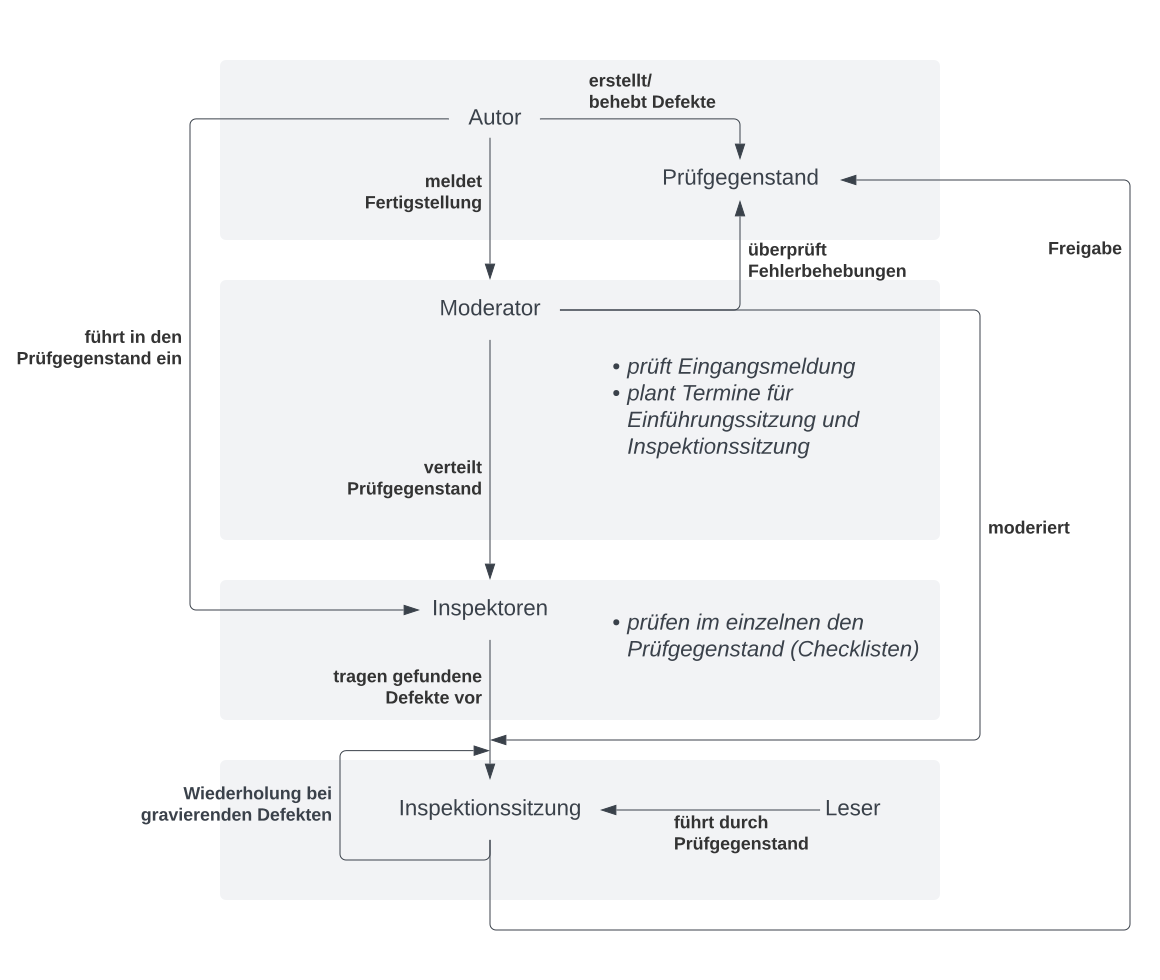
\includegraphics[scale=0.4]{part four/Manuelle Verfahren/img/inspektion}
    \caption{Skizzenhafte Darstellung des Ablaufs von Inspektionen und der damit verbundenen Rollen und ihrer Aufgaben. Nicht aufgeführt in der Darstellung ist die Protokollierung, die in kleineren Gruppen der Moderator übernimmt, ansonsten ein dedizierter Protokollführer. (Quelle: eigene)}
    \label{fig:inspektion}
\end{figure}


\noindent
Eine Gefahr für den Erfolg von Inspektionssitzungen ist gegeben dadurch, dass Inspektoren die Defekte nicht in der Inspektionssitzung bekannt geben, um den \textbf{Autor} nicht zu kritisieren.\\
Im Gegenzug erwarten sie, dass der Autor sie in einer anderen Inspektion nicht kritisiert.\\
Dies lässt sich vermeiden, indem

\begin{itemize}
    \item die Ergebnisse von Inspektionen nicht dazu verwendet werden, den Autor zu beurteilen
    \item ausschließlich der Prüfgegenstand beurteilt wird
    \item das Management die Ergebnisse von Inspektionssitzungen nicht in Zielvorgaben mit dem Autor einfließen lässt
    \item keine Vorgesetzten in der Inspektionssitzung anwesend sind
    \item der Moderator darauf achtet, dass die Inspektoren ausschließlich den Prüfgegenstand kritisieren, nicht den Autor
    \item der Autor nur Fragen beantwortet und keine Möglichkeit erhält, sich für Defekte zu rechtfertigen
\end{itemize}

\subsection{Dokumentation}
Prinzipiell sind \textbf{zwei Protokolle} zu erstellen:

\begin{enumerate}
    \item das erste Protokoll dient dazu, \textbf{Ergebnisse der Inspektionssitzung} festzuhalten.\\
    Es enthält Daten der Sitzung, sowie der gefundenen Defekte mit einer kurzen Beschreibung und der Schwere.
    \item das zweite Protokoll enthält Daten, um die Inspektion \textbf{statistisch auszuwerten}. \\
    Bspw. wird der Prüfumfang notiert, sowie die beteiligten Inspektoren (anonymisiert) und ihre aufgewendete Zeit und die Anzahl der von ihnen gefundenen (schweren) Defekte gelistet; hierdurch läßt sich der Gesamtaufwand und die Effektivität ermitteln (vgl.~\cite[Abb. 3.2, 22]{Wed09c}).\\
    Diese Art der Protokolle helfen dem \textbf{Projektleiter} bei der Beurteilung hinsichtlich der Effektivität der Maßnahmen, und ob in einem Projekt viele Defekte gefunden worden sind.
\end{enumerate}

\noindent
Die bereits erwähnten \textbf{Checklisten} sind Dokumente mit Listen von typischen Defekten, die dabei helfen können, systematisch die Defekte von Prüfgegenständen zu finden.\\
Ein Beispiel für eine typische Checkliste zur Überprüfung von \textbf{Klassenmodellen} gibt \textit{Wedemann} in \cite[Abb. 3.3, 23]{Wed09c} an (s. Tabelle~\ref{tab:checkliste})

% Please add the following required packages to your document preamble:
% \usepackage[table,xcdraw]{xcolor}
% Beamer presentation requires \usepackage{colortbl} instead of \usepackage[table,xcdraw]{xcolor}
\begin{table}[]
    \begin{tabular}{|l|l|}
        \hline
        \rowcolor[HTML]{C0C0C0}
        \textbf{Gegenstand} & \multicolumn{1}{c|}{\cellcolor[HTML]{C0C0C0}\textbf{Überprüfen}}                                                                                    \\ \hline
        Klassen             & \begin{tabular}[c]{@{}l@{}}Kein Objekt?\\ Name: Geeignet? Prägnant? Substantiv? Singular?\end{tabular}                                              \\ \hline
        Attribute           & \begin{tabular}[c]{@{}l@{}}Notwendig?\\ Elementarer Datentyp?\\ Keine Existenz unabhängig vom Objekt?\\ Geeigneter Name?\end{tabular}               \\ \hline
        Assoziation         & \begin{tabular}[c]{@{}l@{}}Geeignet?\\ Multiplizität sinnvoll?\end{tabular}                                                                         \\ \hline
        Vererbung           & \begin{tabular}[c]{@{}l@{}}Besser Komposition anstelle von Vererbung?\\ Kann die Superklasse durch abgeleitete Klassen ersetzt werden?\end{tabular} \\ \hline
    \end{tabular}
    \caption{Beispiel für eine Checkliste zur Prüfung eines Klassenmodells. (Quelle: in Anlehnung an \cite[Abb 3.3, 23]{Wed09c})}\label{tab:checkliste}
\end{table}















